% !TEX TS-program = pdflatex
% !TEX encoding = UTF-8 Unicode

%%% DOCUMENT DEFINITION
\documentclass[11pt, french]{article} % use larger type; default would be 10pt
\usepackage[utf8]{inputenc} % set input encoding (not needed with XeLaTeX)

%%% PAGE DIMENSIONS
\usepackage{geometry} % to change the page dimensions
\geometry{a4paper} % or letterpaper (US) or a5paper or....
\geometry{margin=1in} % for example, change the margins to 2 inches all round

%%% PACKAGES
\usepackage{graphicx} % support the \includegraphics command and options
\usepackage{booktabs} % for much better looking tables
\usepackage{array} % for better arrays (eg matrices) in maths
\usepackage{paralist} % very flexible & customisable lists (eg. enumerate/itemize, etc.)
\usepackage{verbatim} % adds environment for commenting out blocks of text & for better verbatim
\usepackage{subfig} % make it possible to include more than one captioned figure/table in a single float
\usepackage[frenchb]{babel}

% Package pour le dessin schéma bloc
\graphicspath{{../Automatique/}}
\usepackage{schemabloc}
\usepackage{amsmath}

%%% HEADERS & FOOTERS
%\usepackage{fancyhdr} % This should be set AFTER setting up the page geometry
%\pagestyle{fancy} % options: empty , plain , fancy

% Rapport projet pluridisciplinaire
% : Xavier Galzin, Stanislas Bertrand, Romain Desille, Frédéric Meslin

\title{Projet pluridisciplinaire : sustentation magnétique}
\author{Xavier GALZIN, Stanislas BERTRAND, Romain DESILLE, Frédéric MESLIN}
\date{30/01/2012}

\begin{document}
\maketitle

\begin{center}
	\vspace{0.6in}
	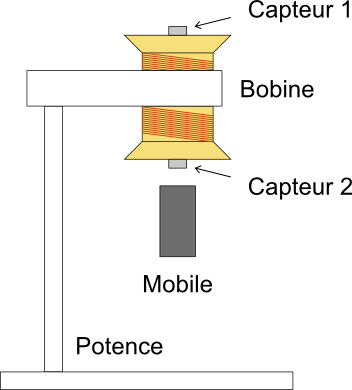
\includegraphics[width=10cm]{Automatique/system_physique.png} 
	\\
	\emph{Le système physique étudié}
\end{center}

\pagebreak

\section{Introduction}
\paragraph{}
Dans le cadre du projet pluridisciplinaire de cette année, il nous est demandé de faire léviter un mobile dans l'air à l'aide d'un champ magnétique produit par une bobine. On appelle cet effet la sustentation magnétique. Ce projet est une version édulcorée d'un prototype de lampe décorative imaginée par une étudiante de l'école LISAA (Institut supérieur des arts appliqués) et réalisée en partenariat avec des chercheurs et ingénieurs de l'INSA de Rennes.

L'étude demandée présente de nombreuses facettes : il faudra d'abord décrire et modéliser le système physique pour ensuite l'asservir à l'aide d'un dispositif automatique électronique. Ce dispositif sera réalisé de manière analogique puis de manière numérique. Dans ce rapport, nous nous intéresserons uniquement à la partie automatique, nous expliquerons la modélisation choisie ainsi que les correcteurs et leurs paramètres clefs pour faire léviter le mobile.

\section{Description du système physique}
\paragraph{}

Le système physique est existant et imposé. Il consiste en une potence munie d'une bobine qui servira à exercer le champs magnétique retenant le mobile. La bobine est également munie de capteurs à effet Hall qui permettent, par une mesure différentielle, de mesurer la distance du mobile par rapport à la bobine. Nous avons ainsi la boucle de retour de notre système. 

Nous avons donc finalement une consigne en position que nous allons convertir en un courant qui servira à générer le champs magnétique qui attirera ou repoussera le mobile et le retour en position par le biais des capteurs à effet Hall. 

Le problème principal du système est qu'il n'est pas stable en boucle ouverte. Nous allons donc procéder à une étude basée sur des mesures fournies afin de mettre en place un correcteur qui rendra la système stable. Pour cela, nous poserons les équations mathématiques du problème pour ensuite décrire le modèle de correcteur retenu ainsi que les valeurs des diverses constantes associées à ce modèle.

\section{Modélisation mathématique}

\paragraph{}
\textsc{Mise en équation du système}

\noindent
Bilan des forces appliquées sur le système :

\smallskip
$ F_{bobine} = K \times \dfrac{i^2}{x^2}  $

$ F_{poids} = -m \times g $

$ F_{perturbations} $
 \medskip

\noindent
Pour simplifier le calcul, on considèrera en premier lieu que les perturbations sont nulles.
On applique ensuite le principe fondamental de la dynamique :

 \medskip
$ \sum F_{exterieures}  = m \times {\dfrac{{d^2}x}{dt^2}} $
 \medskip

\noindent
Résoudre cette équation différentielle est complexe car l'expression de la force de la bobine n'est pas linéaire et elle dépend de deux paramètres du système (i et x) indépendants. On choisit donc de la linéariser (ordre 1) autour du point d'équilibre ($I_0, X_0 $) à l'aide de la différentielle de la fonction.
Linéarisation de la force exercée par la bobine :

 \medskip
$ {\dfrac{dF(t)}{dt}}_{x = X_0, i = I_0} = \dfrac{\partial F(t)}{\partial x} \times dx + \dfrac{\partial F(t)}{\partial i} \times di $
 \medskip

\noindent
On introduit deux coefficients $ K_x $ et $ K_i $ qui correspondent respectivement aux dérivées partielles suivant x et i de F.

 \medskip
$ \dfrac{\partial F(t)}{\partial x} = K_x = \dfrac{-2K \times I_0^2}{X_0^3} $

$ \dfrac{\partial F(t)}{\partial i} = K_i = \dfrac{2K \times I_0}{X_0^2} $
 \medskip

\noindent
On obtient avec la linéarisation l'équation différentielle suivante :

 \medskip
$ m \times {\dfrac{{d^2}x}{dt^2}} = F_{bobine} - m \times g = K \times {\dfrac{I_0^2}{X_0^2}} + K_x \times Dx + K_i \times Di - m \times g $
 \medskip

$ avec : Dx = x - X_0, Di = i - I_0 $
 \medskip

\noindent
On transfert ensuite l'équation dans le domaine de Laplace :

 \medskip
$ m \times x{s^2} = F_0 + K_x \times (x - X_0) + K_i \times (i - I_0) - m \times g $

$ x \times (m{s^2} - K_x) = K_i \times i +(F_0 - K_x \times X_0 - K_i \times I_0 - m \times g) $
 \medskip

\noindent
On remarque que $K_x \times X_0 $ et $K_i \times  I_0$ se compensent et que $ F_0 $ est égale à $ m \times g $. On obtient donc la fonction de transfert suivante :

 \medskip
$ \rightarrow H(s) = \dfrac{x(s)}{i(s)} = \dfrac{K_i}{m{s^2}- K_x}  $
 \medskip

\noindent
K étant jusqu'à présent inconnue, on utilise l'équation du système à l'équilibre et les couples de valeurs mesurées autour du point $ X_0  $ et $ I_0 $ :

 \medskip
$ \sum F_{exterieures}  = K \times {\dfrac{I_0^2}{X_0^2}} - m \times g = 0 $

$ K = mg \times {\dfrac{X_0^2}{I_0^2}} $

\paragraph{}
\textsc{Constantes mécaniques obtenues}

\noindent
En prenant les mesures données et en étudiant le mobile avec son leste, on obtient  :

\medskip
\begin{tabular} {|l|c|r|}
	 \hline
	\textbf{Distance (mm)} & \textbf{Courant (A)} & \textbf{K (calculé)} \\ \hline
	14 & 1.21 & $ 1,857 \times 10^{-4} $ \\ \hline
	15 & 1.48 & $ 1,425  \times 10^{-4} $ \\ \hline
	16 & 1.8 & $ 1,096  \times 10^{-4} $ \\ \hline
\end{tabular}

\medskip
\noindent
En faisant une moyenne des K, on trouve :

\medskip
$ \rightarrow K_{bobine} = 1,459 \times 10^{-4} $
$ \rightarrow K_x = 141,7 $
$ \rightarrow K_i = 1,660 $

\paragraph{}
\textsc{Autres constantes du système}

\medskip
$  \tau_{elec} = \dfrac L R = 6,643 \times 10^{-3} s.rad^{-1} $

$  \tau_{meca} = \dfrac m {K_x} = 9,980 \times 10^{-1} s.rad^{-1} $

\medskip
$  K_{elec} = \dfrac 1 R = 4,464 \times 10^{-1} $

$  K_{hall} = 36,5 V.m^{-1} $

\medskip
La plupart de ces valeurs ont été obtenues par calcul direct alors que le gain $ K_{hall} $ a été déterminée à l'aide d'une opération de régression linéaire sur la courbe de la tension différentielle des capteurs ($ V_{H2} - V_{H1} $) en fonction de la distance du mobile.

\section{Correcteur analogique}
\subsection{Choix du correcteur}
Dans un premier temps, nous avons choisi un correcteur proportionnel-dérivé. Un correcteur dérivé n'étant pas réalisable physiquement, nous allons donc le remplacer par un correcteur à avance de phase.

\medskip
En traçant le diagramme de Black - Nichols du système non corrigé, on s'aperçoit que celui ci est instable en boucle ouverte car en $\omega = 0$ le système est déphasé de 180\char23. Nous allons donc tenté de réduire le déphase du système afin de pouvoir passer à droite du point 180\char23.

\medskip
\begin{center}
\begin{tikzpicture}
\sbEntree{Vxc}
\sbComp{Comp}{Vxc}
	\sbRelier[$Vx_C$]{Vxc}{Comp}
\sbBloc{C}{$K_{p}$}{Comp}
	\sbRelier[$\epsilon_x$]{Comp}{C}
\sbBlocL{E}{$\dfrac{K_{Elec}}{\tau_{Elec} \cdot p + 1}$}{C} 
\sbBlocL{M}{$\dfrac{-\frac{K_i}{K_x}}{-{\tau_{Meca}}^2 \cdot p^2 - 1}$}{E}
\sbBlocL{H}{$K_{Hall}$}{M} 

\sbSortie{Vxr}{H} 
	\sbRelier{H}{Vxr}
	\sbNomLien[0.8]{Vxr}{$Vx_R$} 
\sbDecaleNoeudy{M}{A}
\sbBlocr[0]{A}{$\dfrac{1+ \tau_d \cdot p}{1 + a_d \cdot \tau_d \cdot p}$}{A}
\sbRelieryx{H-Vxr}{A}
\sbRelierxy{A}{Comp}
\end{tikzpicture}

$\tau_d = $


\hspace{1mm} \\ 
\hspace{1mm}\textcolor{green}{\% Paramètres du Système }\\ 
\hspace{1mm} \\ 
\hspace{1mm}\textcolor{green}{\% Modèle Electrique de la Bobine }\\ 
\hspace{1mm}R=2.24; \textcolor{green}{\%Ohm }\\ 
\hspace{1mm}L=1.49e-2; \textcolor{green}{\%H }\\ 
\hspace{1mm} \\ 
\hspace{1mm}\textcolor{green}{\% Modèle d'interaction mécanique de la bobine }\\ 
\hspace{1mm}m=0.1414; \textcolor{green}{\%Kg }\\ 
\hspace{1mm}ki=1.375; \textcolor{green}{\%N.A-1 }\\ 
\hspace{1mm}kx=117.3; \textcolor{green}{\%N.m-1 }\\ 
\hspace{1mm} \\ 
\hspace{1mm}\textcolor{green}{\% Modèle capteur effet Hall }\\ 
\hspace{1mm}Kc\_Hall=92;  \\ 
\hspace{1mm} \\ 


\emph{Schéma bloc du système complet avec correcteur}
\end{center}

\subsection{Choix des constantes}

Pour choisir les constantes du correcteur, nous avons procédé en deux étapes. Premièrement, nous avons réglé le correcteur à avance de phase. Pour cela, nous nous sommes servis du lieu d'Evans. On peut remarquer que, quelque soit le gain du correcteur, au moins un des pôles du système restera à droite de l'axe des imaginaires.

\begin{center}
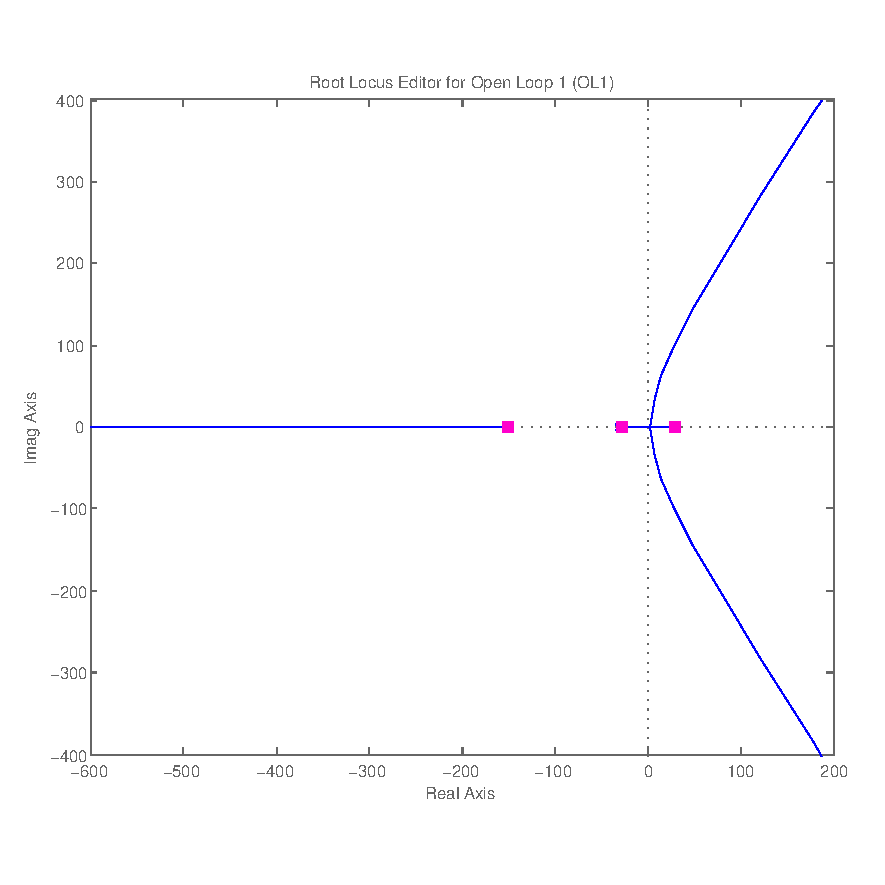
\includegraphics [scale=0.50]{RL_Sys_Seul.pdf}
\\
\emph{Lieu d'Evans du système non corrigé}
\end{center}

L'idée est donc de décaler le point d'intersection des asymptotes qui est normalement dans la partie droite du plan complexe en plaçant le zéros du correcteur à avance de phase dans la partie gauche tout en maintenant ce zéro avant le pôle issu de la constante de temps mécanique qui se trouve dans la partie gauche. Une fois que la position des asymptotes a été correcte, nous avons réglé le gain du correcteur proportionnel afin que tous les pôles du système se retrouvent à droite de l'axe des imaginaires. Nous avons trouvé un gain K de 5. 

\begin{center}
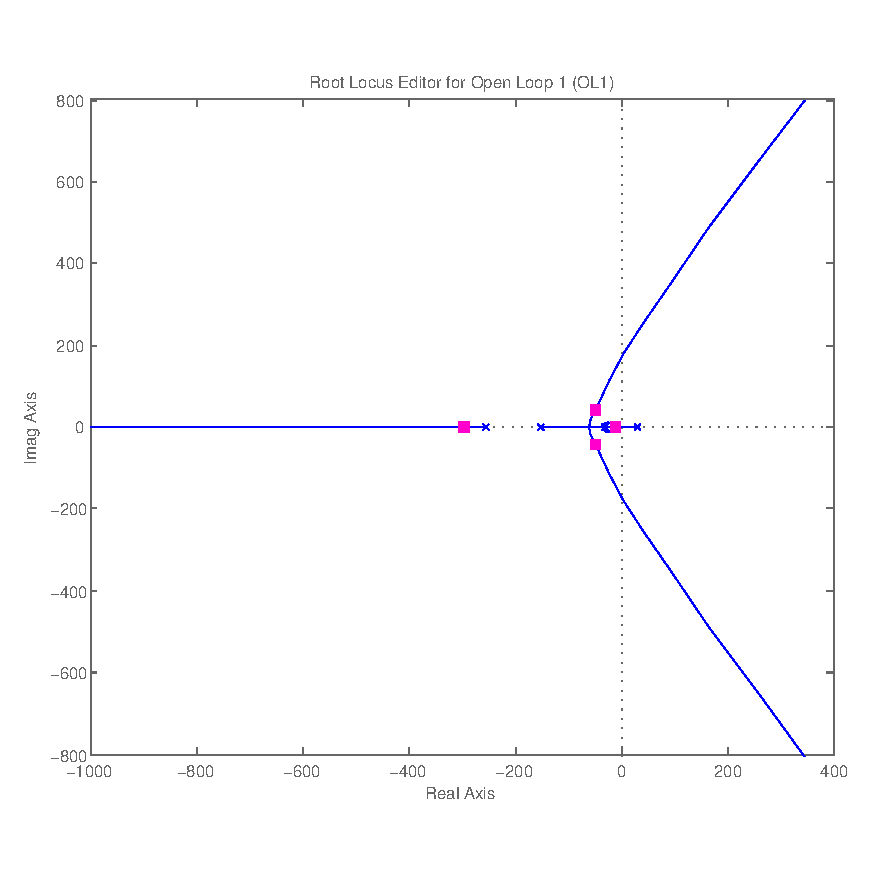
\includegraphics[scale=0.50]{RL_Sys_AvPh_K10.pdf}
\\
\emph{Lieu d'Evans du système corrigé}
\end{center}

Nous avons ensuite tracé le diagramme de Black - Nichols du système corrigé afin de vérifier les marges de gain et de phase. Cela nous a permis d'obtenir une marge de phase d'environ 25\char23 et une marge de gain de plus de 10 dB.

\begin{center}
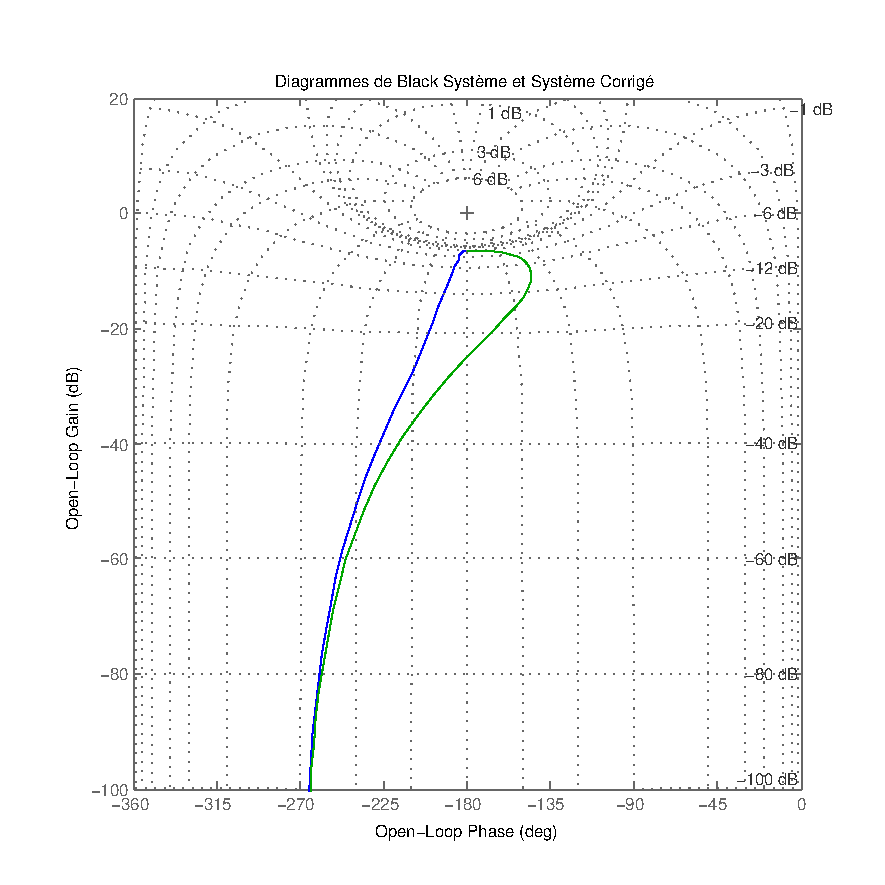
\includegraphics[scale=0.50]{MatBlackFredValues.pdf}
\\
\emph{Diagramme de Black-Nichols du système corrigé}
\end{center}

\section{Correcteur numérique}

Dans la seconde partie du projet, nous commencerons par simplement convertir notre correcteur analogique par le biais d'une approximation des rectangles avant. Nous avons choisi cette solution car elle est réalisable physiquement contrairement à celle des rectangles arrière. En outre, elle est assez précise et plus facile à mettre en oeuvre que l'approximation de Tustin. Dans l'absolu, rien ne nous empêchera de changer cette approximation par la suite dans le cas où les résultats seraient insatisfaisants. 

L'équation du système par l'approximation des rectangle avant devient :

$  H_{système} = \dfrac {4.957\times 10^{-5}z^{2} + 1.86\times 10^{-4}z + 4.349\times 10^{-5}} {z^{3} - 2.772z^{2} + 2.541z - 0.7697} $
\medskip

$  H_{correcteur} = \dfrac {8.356z - 8.014} {z - 0.6584} $
\medskip
 
\begin{center}
\begin{tikzpicture}
\sbEntree{Vxc}
\sbComp{Comp}{Vxc}
	\sbRelier[$Vx_C$]{Vxc}{Comp}
\sbBloc{C}{$K_{p}$}{Comp}
	\sbRelier[$\epsilon_x$]{Comp}{C}
\sbBlocL{E}{$\dfrac{K_{Elec}}{\tau_{Elec} \cdot p + 1}$}{C} 
\sbBlocL{M}{$\dfrac{-\frac{K_i}{K_x}}{-{\tau_{Meca}}^2 \cdot p^2 - 1}$}{E}
\sbBlocL{H}{$K_{Hall}$}{M} 

\sbSortie{Vxr}{H} 
	\sbRelier{H}{Vxr}
	\sbNomLien[0.8]{Vxr}{$Vx_R$} 
\sbDecaleNoeudy{M}{A}
\sbBlocr[0]{A}{$\dfrac{1+ \tau_d \cdot p}{1 + a_d \cdot \tau_d \cdot p}$}{A}
\sbRelieryx{H-Vxr}{A}
\sbRelierxy{A}{Comp}
\end{tikzpicture}

%$\tau_d = $
%\hspace{1mm} \\ 
\hspace{1mm}\textcolor{green}{\% Paramètres du Système }\\ 
\hspace{1mm} \\ 
\hspace{1mm}\textcolor{green}{\% Modèle Electrique de la Bobine }\\ 
\hspace{1mm}R=2.24; \textcolor{green}{\%Ohm }\\ 
\hspace{1mm}L=1.49e-2; \textcolor{green}{\%H }\\ 
\hspace{1mm} \\ 
\hspace{1mm}\textcolor{green}{\% Modèle d'interaction mécanique de la bobine }\\ 
\hspace{1mm}m=0.1414; \textcolor{green}{\%Kg }\\ 
\hspace{1mm}ki=1.375; \textcolor{green}{\%N.A-1 }\\ 
\hspace{1mm}kx=117.3; \textcolor{green}{\%N.m-1 }\\ 
\hspace{1mm} \\ 
\hspace{1mm}\textcolor{green}{\% Modèle capteur effet Hall }\\ 
\hspace{1mm}Kc\_Hall=92;  \\ 
\hspace{1mm} \\ 


\emph{Schéma bloc du système complet avec correcteur (Réprésentation en Numérique}
\end{center}

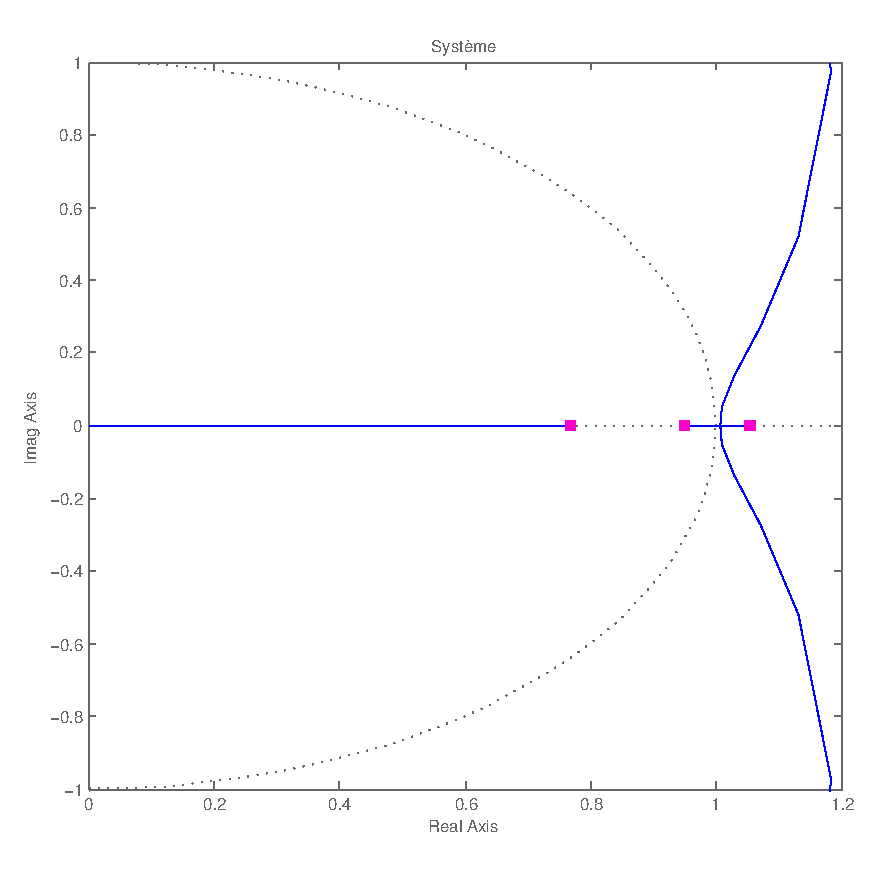
\includegraphics[scale=0.50]{RLN_Sys_Seul.pdf}
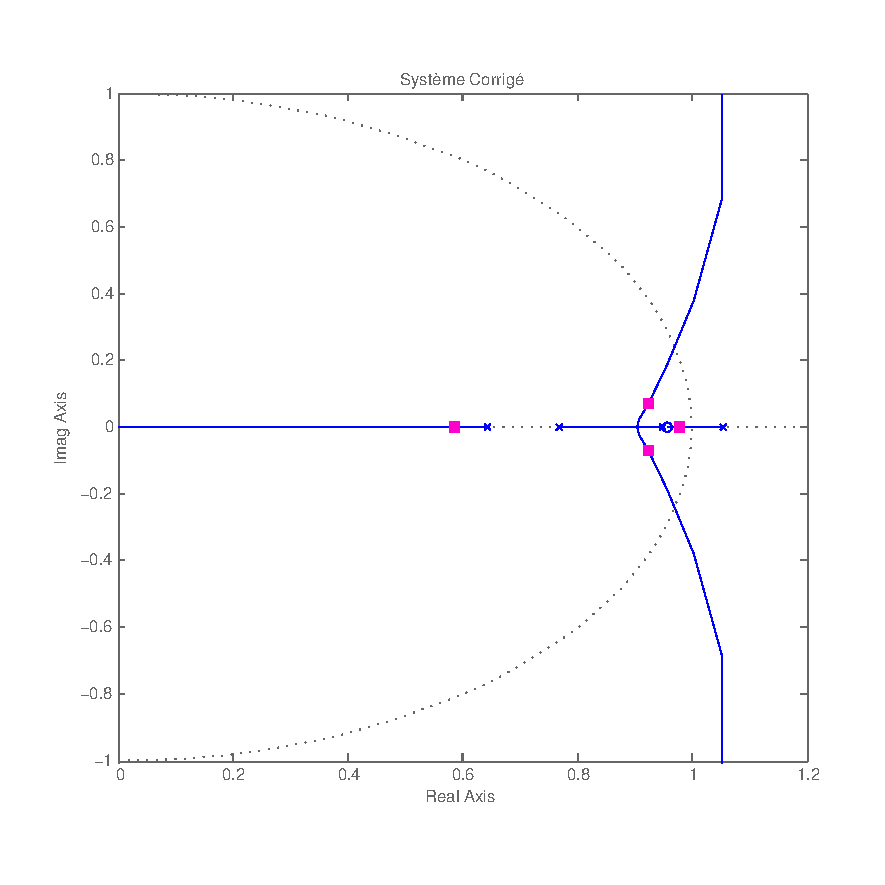
\includegraphics[scale=0.50]{RLN_Sys_AvPh_K10.pdf}

\section{Conclusion}

Grâce à cette étude, nous avons pu trouver des valeurs de paramètres de correcteurs qui nous permettent de stabiliser le système. Cependant, nous pouvons nous interroger sur la fiabilité de ces paramètres étant donné qu'ils sont basés sur une approximation linéaire du système. De même, le modèle du champs magnétique pourrait se révéler trop imprécis et ainsi fausser le calcul des constantes. Il faudra donc garder cela à l'esprit pour éventuellement réévaluer nos paramètres par la suite. 

\end{document}
